\documentclass{beamer}
\usetheme{metropolis}
\usepackage{tikz}
\usepackage[none]{hyphenat}

\title{Keynesians to the Rescue: Unprecedented Policy Responses Towards Unprecedented Macroeconomic Shocks (Evidence from Three Natural Experiments)}
\subtitle{Lille Post-Keynesian Conference 
\newline December 6-8, 2023 }
\date{Dec 6, 2023}
\author{Lyuben Ivanov, PhD}
\institute{Faculty of Economics and Business, Sofia University St. Kliment Ohridski}

\begin{document}

\maketitle

\section{Fiscal and Monetary Responses to Three Major Macroeconomic Shocks}

\begin{frame}{Fiscal Response to the GFC and the COVID-19 Pandemic}

\begin{figure}[h!]
     \centering
     % Created by tikzDevice version 0.12.5 on 2023-11-24 22:18:14
% !TEX encoding = UTF-8 Unicode
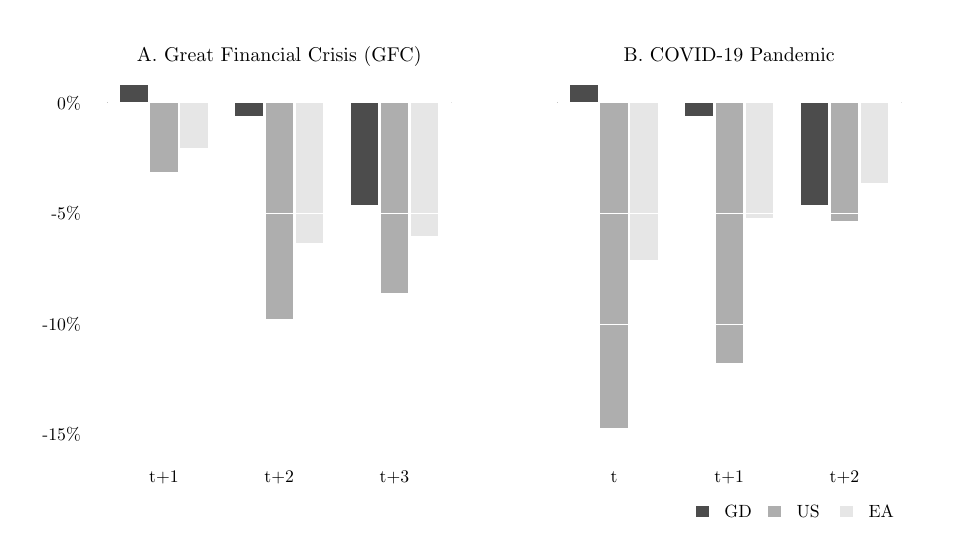
\begin{tikzpicture}[x=1pt,y=1pt]
\definecolor{fillColor}{RGB}{255,255,255}
\path[use as bounding box,fill=fillColor,fill opacity=0.00] (0,0) rectangle (325.21,180.67);
\begin{scope}
\path[clip] (  0.00,  0.00) rectangle (162.61,180.67);
\definecolor{fillColor}{gray}{0.30}

\path[fill=fillColor] ( 33.40,153.48) rectangle ( 43.31,159.88);
\definecolor{fillColor}{RGB}{174,174,174}

\path[fill=fillColor] ( 44.31,153.48) rectangle ( 54.22,128.67);
\definecolor{fillColor}{RGB}{230,230,230}

\path[fill=fillColor] ( 55.21,153.48) rectangle ( 65.13,137.14);
\definecolor{fillColor}{gray}{0.30}

\path[fill=fillColor] ( 75.04,153.48) rectangle ( 84.96,148.71);
\definecolor{fillColor}{RGB}{174,174,174}

\path[fill=fillColor] ( 85.95,153.48) rectangle ( 95.86, 75.50);
\definecolor{fillColor}{RGB}{230,230,230}

\path[fill=fillColor] ( 96.85,153.48) rectangle (106.77,102.79);
\definecolor{fillColor}{gray}{0.30}

\path[fill=fillColor] (116.68,153.48) rectangle (126.60,116.76);
\definecolor{fillColor}{RGB}{174,174,174}

\path[fill=fillColor] (127.59,153.48) rectangle (137.50, 84.74);
\definecolor{fillColor}{RGB}{230,230,230}

\path[fill=fillColor] (138.49,153.48) rectangle (148.41,105.51);
\end{scope}
\begin{scope}
\path[clip] (  0.00,  0.00) rectangle (325.21,180.67);
\definecolor{drawColor}{RGB}{0,0,0}

\node[text=drawColor,anchor=base,inner sep=0pt, outer sep=0pt, scale=  0.64] at ( 49.26, 16.32) {t+1};

\node[text=drawColor,anchor=base,inner sep=0pt, outer sep=0pt, scale=  0.64] at ( 90.90, 16.32) {t+2};

\node[text=drawColor,anchor=base,inner sep=0pt, outer sep=0pt, scale=  0.64] at (132.54, 16.32) {t+3};
\end{scope}
\begin{scope}
\path[clip] ( 28.80, 33.60) rectangle (153.01,161.47);
\definecolor{drawColor}{RGB}{0,0,0}

\path[draw=drawColor,line width= 0.4pt,line join=round,line cap=round] ( 28.80,153.48) -- (153.01,153.48);
\end{scope}
\begin{scope}
\path[clip] (  0.00,  0.00) rectangle (325.21,180.67);
\definecolor{drawColor}{RGB}{0,0,0}

\node[text=drawColor,anchor=base east,inner sep=0pt, outer sep=0pt, scale=  0.64] at ( 19.20, 31.40) {-15\%};

\node[text=drawColor,anchor=base east,inner sep=0pt, outer sep=0pt, scale=  0.64] at ( 19.20, 71.36) {-10\%};

\node[text=drawColor,anchor=base east,inner sep=0pt, outer sep=0pt, scale=  0.64] at ( 19.20,111.32) {-5\%};

\node[text=drawColor,anchor=base east,inner sep=0pt, outer sep=0pt, scale=  0.64] at ( 19.20,151.28) {0\%};
\end{scope}
\begin{scope}
\path[clip] ( 28.80, 33.60) rectangle (153.01,161.47);
\definecolor{drawColor}{RGB}{255,255,255}

\path[draw=drawColor,line width= 0.4pt,line join=round,line cap=round] ( 28.80, 33.60) -- (153.01, 33.60);

\path[draw=drawColor,line width= 0.4pt,line join=round,line cap=round] ( 28.80, 73.56) -- (153.01, 73.56);

\path[draw=drawColor,line width= 0.4pt,line join=round,line cap=round] ( 28.80,113.52) -- (153.01,113.52);

\path[draw=drawColor,line width= 0.4pt,line join=round,line cap=round] ( 28.80,153.48) -- (153.01,153.48);
\end{scope}
\begin{scope}
\path[clip] (  0.00,  0.00) rectangle (162.61,180.67);
\definecolor{drawColor}{RGB}{0,0,0}

\node[text=drawColor,anchor=base,inner sep=0pt, outer sep=0pt, scale=  0.72] at ( 90.90,168.60) {A. Great Financial Crisis (GFC)};
\end{scope}
\begin{scope}
\path[clip] (162.61,  0.00) rectangle (325.21,180.67);
\definecolor{fillColor}{gray}{0.30}

\path[fill=fillColor] (196.01,153.48) rectangle (205.92,159.88);
\definecolor{fillColor}{RGB}{174,174,174}

\path[fill=fillColor] (206.91,153.48) rectangle (216.83, 36.07);
\definecolor{fillColor}{RGB}{230,230,230}

\path[fill=fillColor] (217.82,153.48) rectangle (227.73, 96.74);
\definecolor{fillColor}{gray}{0.30}

\path[fill=fillColor] (237.65,153.48) rectangle (247.56,148.71);
\definecolor{fillColor}{RGB}{174,174,174}

\path[fill=fillColor] (248.55,153.48) rectangle (258.47, 59.47);
\definecolor{fillColor}{RGB}{230,230,230}

\path[fill=fillColor] (259.46,153.48) rectangle (269.37,111.92);
\definecolor{fillColor}{gray}{0.30}

\path[fill=fillColor] (279.29,153.48) rectangle (289.20,116.76);
\definecolor{fillColor}{RGB}{174,174,174}

\path[fill=fillColor] (290.19,153.48) rectangle (300.11,110.78);
\definecolor{fillColor}{RGB}{230,230,230}

\path[fill=fillColor] (301.10,153.48) rectangle (311.01,124.71);
\end{scope}
\begin{scope}
\path[clip] (  0.00,  0.00) rectangle (325.21,180.67);
\definecolor{drawColor}{RGB}{0,0,0}

\node[text=drawColor,anchor=base,inner sep=0pt, outer sep=0pt, scale=  0.64] at (211.87, 16.32) {t};

\node[text=drawColor,anchor=base,inner sep=0pt, outer sep=0pt, scale=  0.64] at (253.51, 16.32) {t+1};

\node[text=drawColor,anchor=base,inner sep=0pt, outer sep=0pt, scale=  0.64] at (295.15, 16.32) {t+2};
\end{scope}
\begin{scope}
\path[clip] (191.41, 33.60) rectangle (315.62,161.47);
\definecolor{drawColor}{RGB}{0,0,0}

\path[draw=drawColor,line width= 0.4pt,line join=round,line cap=round] (191.41,153.48) -- (315.62,153.48);
\definecolor{drawColor}{RGB}{255,255,255}

\path[draw=drawColor,line width= 0.4pt,line join=round,line cap=round] (191.41, 33.60) -- (315.62, 33.60);

\path[draw=drawColor,line width= 0.4pt,line join=round,line cap=round] (191.41, 73.56) -- (315.62, 73.56);

\path[draw=drawColor,line width= 0.4pt,line join=round,line cap=round] (191.41,113.52) -- (315.62,113.52);

\path[draw=drawColor,line width= 0.4pt,line join=round,line cap=round] (191.41,153.48) -- (315.62,153.48);
\end{scope}
\begin{scope}
\path[clip] (162.61,  0.00) rectangle (325.21,180.67);
\definecolor{fillColor}{gray}{0.30}

\path[fill=fillColor] (241.43,  7.86) rectangle (246.03,  4.02);
\definecolor{fillColor}{RGB}{174,174,174}

\path[fill=fillColor] (267.46,  7.86) rectangle (272.07,  4.02);
\definecolor{fillColor}{RGB}{230,230,230}

\path[fill=fillColor] (293.50,  7.86) rectangle (298.11,  4.02);
\definecolor{drawColor}{RGB}{0,0,0}

\node[text=drawColor,anchor=base west,inner sep=0pt, outer sep=0pt, scale=  0.64] at (251.79,  3.74) {GD};

\node[text=drawColor,anchor=base west,inner sep=0pt, outer sep=0pt, scale=  0.64] at (277.83,  3.74) {US};

\node[text=drawColor,anchor=base west,inner sep=0pt, outer sep=0pt, scale=  0.64] at (303.87,  3.74) {EA};

\node[text=drawColor,anchor=base,inner sep=0pt, outer sep=0pt, scale=  0.72] at (253.51,168.60) {B. COVID-19 Pandemic};
\end{scope}
\end{tikzpicture}

\end{figure} 
	
\end{frame}

\begin{frame}{Monetary Response to the GFC and the COVID-19 Pandemic}

\begin{figure}[h!]
     \centering
     % Created by tikzDevice version 0.12.5 on 2023-11-24 22:28:42
% !TEX encoding = UTF-8 Unicode
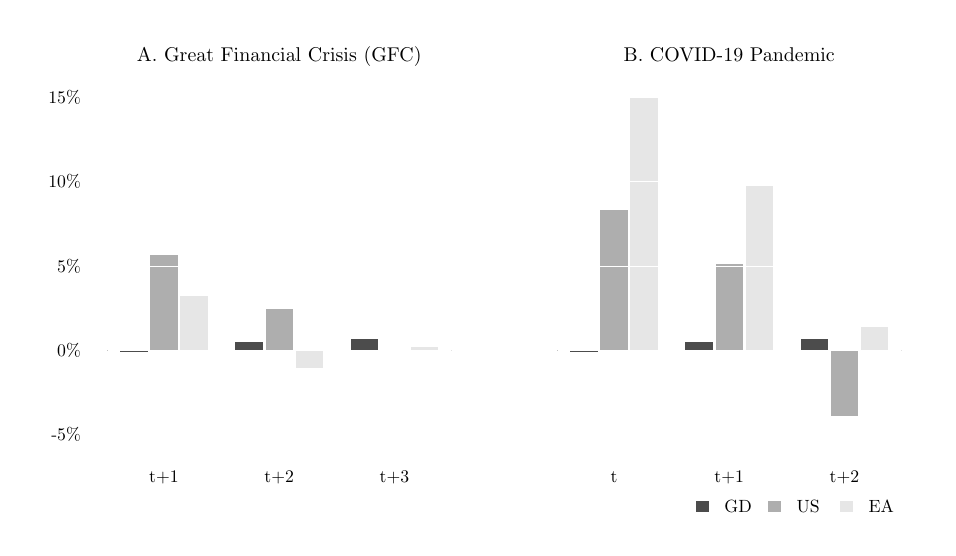
\begin{tikzpicture}[x=1pt,y=1pt]
\definecolor{fillColor}{RGB}{255,255,255}
\path[use as bounding box,fill=fillColor,fill opacity=0.00] (0,0) rectangle (325.21,180.67);
\begin{scope}
\path[clip] (  0.00,  0.00) rectangle (162.61,180.67);
\definecolor{fillColor}{gray}{0.30}

\path[fill=fillColor] ( 33.40, 64.05) rectangle ( 43.31, 63.46);
\definecolor{fillColor}{RGB}{174,174,174}

\path[fill=fillColor] ( 44.31, 64.05) rectangle ( 54.22, 98.40);
\definecolor{fillColor}{RGB}{230,230,230}

\path[fill=fillColor] ( 55.21, 64.05) rectangle ( 65.13, 83.59);
\definecolor{fillColor}{gray}{0.30}

\path[fill=fillColor] ( 75.04, 64.05) rectangle ( 84.96, 67.13);
\definecolor{fillColor}{RGB}{174,174,174}

\path[fill=fillColor] ( 85.95, 64.05) rectangle ( 95.86, 78.89);
\definecolor{fillColor}{RGB}{230,230,230}

\path[fill=fillColor] ( 96.85, 64.05) rectangle (106.77, 57.59);
\definecolor{fillColor}{gray}{0.30}

\path[fill=fillColor] (116.68, 64.05) rectangle (126.60, 68.16);
\definecolor{fillColor}{RGB}{174,174,174}

\path[fill=fillColor] (127.59, 64.05) rectangle (137.50, 63.72);
\definecolor{fillColor}{RGB}{230,230,230}

\path[fill=fillColor] (138.49, 64.05) rectangle (148.41, 65.37);
\end{scope}
\begin{scope}
\path[clip] (  0.00,  0.00) rectangle (325.21,180.67);
\definecolor{drawColor}{RGB}{0,0,0}

\node[text=drawColor,anchor=base,inner sep=0pt, outer sep=0pt, scale=  0.64] at ( 49.26, 16.32) {t+1};

\node[text=drawColor,anchor=base,inner sep=0pt, outer sep=0pt, scale=  0.64] at ( 90.90, 16.32) {t+2};

\node[text=drawColor,anchor=base,inner sep=0pt, outer sep=0pt, scale=  0.64] at (132.54, 16.32) {t+3};
\end{scope}
\begin{scope}
\path[clip] ( 28.80, 33.60) rectangle (153.01,161.47);
\definecolor{drawColor}{RGB}{0,0,0}

\path[draw=drawColor,line width= 0.4pt,line join=round,line cap=round] ( 28.80, 64.05) -- (153.01, 64.05);
\end{scope}
\begin{scope}
\path[clip] (  0.00,  0.00) rectangle (325.21,180.67);
\definecolor{drawColor}{RGB}{0,0,0}

\node[text=drawColor,anchor=base east,inner sep=0pt, outer sep=0pt, scale=  0.64] at ( 19.20, 31.40) {-5\%};

\node[text=drawColor,anchor=base east,inner sep=0pt, outer sep=0pt, scale=  0.64] at ( 19.20, 61.84) {0\%};

\node[text=drawColor,anchor=base east,inner sep=0pt, outer sep=0pt, scale=  0.64] at ( 19.20, 92.29) {5\%};

\node[text=drawColor,anchor=base east,inner sep=0pt, outer sep=0pt, scale=  0.64] at ( 19.20,122.74) {10\%};

\node[text=drawColor,anchor=base east,inner sep=0pt, outer sep=0pt, scale=  0.64] at ( 19.20,153.18) {15\%};
\end{scope}
\begin{scope}
\path[clip] ( 28.80, 33.60) rectangle (153.01,161.47);
\definecolor{drawColor}{RGB}{255,255,255}

\path[draw=drawColor,line width= 0.4pt,line join=round,line cap=round] ( 28.80, 33.60) -- (153.01, 33.60);

\path[draw=drawColor,line width= 0.4pt,line join=round,line cap=round] ( 28.80, 64.05) -- (153.01, 64.05);

\path[draw=drawColor,line width= 0.4pt,line join=round,line cap=round] ( 28.80, 94.49) -- (153.01, 94.49);

\path[draw=drawColor,line width= 0.4pt,line join=round,line cap=round] ( 28.80,124.94) -- (153.01,124.94);

\path[draw=drawColor,line width= 0.4pt,line join=round,line cap=round] ( 28.80,155.39) -- (153.01,155.39);
\end{scope}
\begin{scope}
\path[clip] (  0.00,  0.00) rectangle (162.61,180.67);
\definecolor{drawColor}{RGB}{0,0,0}

\node[text=drawColor,anchor=base,inner sep=0pt, outer sep=0pt, scale=  0.72] at ( 90.90,168.60) {A. Great Financial Crisis (GFC)};
\end{scope}
\begin{scope}
\path[clip] (162.61,  0.00) rectangle (325.21,180.67);
\definecolor{fillColor}{gray}{0.30}

\path[fill=fillColor] (196.01, 64.05) rectangle (205.92, 63.46);
\definecolor{fillColor}{RGB}{174,174,174}

\path[fill=fillColor] (206.91, 64.05) rectangle (216.83,114.88);
\definecolor{fillColor}{RGB}{230,230,230}

\path[fill=fillColor] (217.82, 64.05) rectangle (227.73,155.23);
\definecolor{fillColor}{gray}{0.30}

\path[fill=fillColor] (237.65, 64.05) rectangle (247.56, 67.13);
\definecolor{fillColor}{RGB}{174,174,174}

\path[fill=fillColor] (248.55, 64.05) rectangle (258.47, 95.19);
\definecolor{fillColor}{RGB}{230,230,230}

\path[fill=fillColor] (259.46, 64.05) rectangle (269.37,123.37);
\definecolor{fillColor}{gray}{0.30}

\path[fill=fillColor] (279.29, 64.05) rectangle (289.20, 68.16);
\definecolor{fillColor}{RGB}{174,174,174}

\path[fill=fillColor] (290.19, 64.05) rectangle (300.11, 40.23);
\definecolor{fillColor}{RGB}{230,230,230}

\path[fill=fillColor] (301.10, 64.05) rectangle (311.01, 72.50);
\end{scope}
\begin{scope}
\path[clip] (  0.00,  0.00) rectangle (325.21,180.67);
\definecolor{drawColor}{RGB}{0,0,0}

\node[text=drawColor,anchor=base,inner sep=0pt, outer sep=0pt, scale=  0.64] at (211.87, 16.32) {t};

\node[text=drawColor,anchor=base,inner sep=0pt, outer sep=0pt, scale=  0.64] at (253.51, 16.32) {t+1};

\node[text=drawColor,anchor=base,inner sep=0pt, outer sep=0pt, scale=  0.64] at (295.15, 16.32) {t+2};
\end{scope}
\begin{scope}
\path[clip] (191.41, 33.60) rectangle (315.62,161.47);
\definecolor{drawColor}{RGB}{0,0,0}

\path[draw=drawColor,line width= 0.4pt,line join=round,line cap=round] (191.41, 64.05) -- (315.62, 64.05);
\definecolor{drawColor}{RGB}{255,255,255}

\path[draw=drawColor,line width= 0.4pt,line join=round,line cap=round] (191.41, 33.60) -- (315.62, 33.60);

\path[draw=drawColor,line width= 0.4pt,line join=round,line cap=round] (191.41, 64.05) -- (315.62, 64.05);

\path[draw=drawColor,line width= 0.4pt,line join=round,line cap=round] (191.41, 94.49) -- (315.62, 94.49);

\path[draw=drawColor,line width= 0.4pt,line join=round,line cap=round] (191.41,124.94) -- (315.62,124.94);

\path[draw=drawColor,line width= 0.4pt,line join=round,line cap=round] (191.41,155.39) -- (315.62,155.39);
\end{scope}
\begin{scope}
\path[clip] (162.61,  0.00) rectangle (325.21,180.67);
\definecolor{fillColor}{gray}{0.30}

\path[fill=fillColor] (241.43,  9.57) rectangle (246.03,  5.73);
\definecolor{fillColor}{RGB}{174,174,174}

\path[fill=fillColor] (267.46,  9.57) rectangle (272.07,  5.73);
\definecolor{fillColor}{RGB}{230,230,230}

\path[fill=fillColor] (293.50,  9.57) rectangle (298.11,  5.73);
\definecolor{drawColor}{RGB}{0,0,0}

\node[text=drawColor,anchor=base west,inner sep=0pt, outer sep=0pt, scale=  0.64] at (251.79,  5.45) {GD};

\node[text=drawColor,anchor=base west,inner sep=0pt, outer sep=0pt, scale=  0.64] at (277.83,  5.45) {US};

\node[text=drawColor,anchor=base west,inner sep=0pt, outer sep=0pt, scale=  0.64] at (303.87,  5.45) {EA};

\node[text=drawColor,anchor=base,inner sep=0pt, outer sep=0pt, scale=  0.72] at (253.51,168.60) {B. COVID-19 Pandemic};
\end{scope}
\end{tikzpicture}

\end{figure} 
	
\end{frame}


\section{Macroeconomic Outcomes}

\begin{frame}{Industrial Production Post GFC and COVID-19 Pandemic}

\begin{figure}[h!]
     \centering
     % Created by tikzDevice version 0.12.5 on 2023-11-24 23:42:35
% !TEX encoding = UTF-8 Unicode
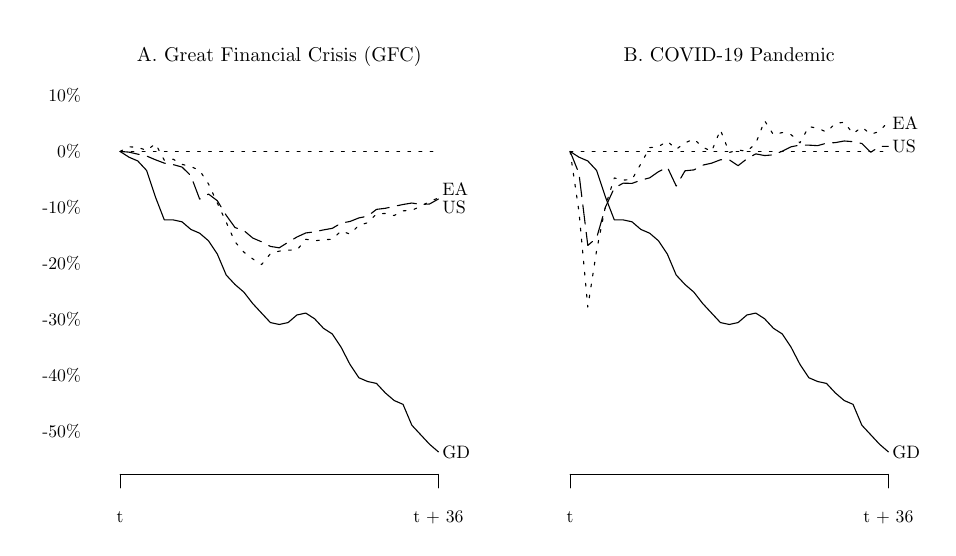
\begin{tikzpicture}[x=1pt,y=1pt]
\definecolor{fillColor}{RGB}{255,255,255}
\path[use as bounding box,fill=fillColor,fill opacity=0.00] (0,0) rectangle (325.21,180.67);
\begin{scope}
\path[clip] ( 28.80, 19.20) rectangle (153.01,161.47);
\definecolor{drawColor}{RGB}{0,0,0}

\path[draw=drawColor,line width= 0.4pt,line join=round,line cap=round] ( 33.40,135.94) --
	( 36.59,133.88) --
	( 39.79,132.50) --
	( 42.98,129.07) --
	( 46.18,119.45) --
	( 49.37,111.21) --
	( 52.57,111.21) --
	( 55.76,110.52) --
	( 58.96,107.77) --
	( 62.15,106.40) --
	( 65.35,103.65) --
	( 68.54, 98.84) --
	( 71.74, 91.28) --
	( 74.93, 87.85) --
	( 78.13, 85.10) --
	( 81.32, 80.98) --
	( 84.51, 77.54) --
	( 87.71, 74.11) --
	( 90.90, 73.42) --
	( 94.10, 74.11) --
	( 97.29, 76.85) --
	(100.49, 77.54) --
	(103.68, 75.48) --
	(106.88, 72.04) --
	(110.07, 69.99) --
	(113.27, 65.17) --
	(116.46, 58.99) --
	(119.66, 54.18) --
	(122.85, 52.81) --
	(126.04, 52.12) --
	(129.24, 48.69) --
	(132.43, 45.94) --
	(135.63, 44.56) --
	(138.82, 37.01) --
	(142.02, 33.57) --
	(145.21, 30.14) --
	(148.41, 27.39);
\end{scope}
\begin{scope}
\path[clip] ( 28.80, 19.20) rectangle (153.01,161.47);
\definecolor{drawColor}{RGB}{0,0,0}

\path[draw=drawColor,line width= 0.4pt,dash pattern=on 1pt off 3pt ,line join=round,line cap=round] ( 33.40,135.94) --
	(148.41,135.94);
\end{scope}
\begin{scope}
\path[clip] (  0.00,  0.00) rectangle (325.21,180.67);
\definecolor{drawColor}{RGB}{0,0,0}

\path[draw=drawColor,line width= 0.4pt,line join=round,line cap=round] ( 33.40, 19.20) -- (148.41, 19.20);

\path[draw=drawColor,line width= 0.4pt,line join=round,line cap=round] ( 33.40, 19.20) -- ( 33.40, 14.40);

\path[draw=drawColor,line width= 0.4pt,line join=round,line cap=round] (148.41, 19.20) -- (148.41, 14.40);

\node[text=drawColor,anchor=base,inner sep=0pt, outer sep=0pt, scale=  0.64] at ( 33.40,  1.92) {t};

\node[text=drawColor,anchor=base,inner sep=0pt, outer sep=0pt, scale=  0.64] at (148.41,  1.92) {t + 36};

\node[text=drawColor,anchor=base east,inner sep=0pt, outer sep=0pt, scale=  0.64] at ( 19.20, 32.40) {-50\%};

\node[text=drawColor,anchor=base east,inner sep=0pt, outer sep=0pt, scale=  0.64] at ( 19.20, 52.67) {-40\%};

\node[text=drawColor,anchor=base east,inner sep=0pt, outer sep=0pt, scale=  0.64] at ( 19.20, 72.93) {-30\%};

\node[text=drawColor,anchor=base east,inner sep=0pt, outer sep=0pt, scale=  0.64] at ( 19.20, 93.20) {-20\%};

\node[text=drawColor,anchor=base east,inner sep=0pt, outer sep=0pt, scale=  0.64] at ( 19.20,113.47) {-10\%};

\node[text=drawColor,anchor=base east,inner sep=0pt, outer sep=0pt, scale=  0.64] at ( 19.20,133.73) {0\%};

\node[text=drawColor,anchor=base east,inner sep=0pt, outer sep=0pt, scale=  0.64] at ( 19.20,154.00) {10\%};

\node[text=drawColor,anchor=base west,inner sep=0pt, outer sep=0pt, scale=  0.65] at (149.84, 25.15) {GD};
\end{scope}
\begin{scope}
\path[clip] ( 28.80, 19.20) rectangle (153.01,161.47);
\definecolor{drawColor}{RGB}{0,0,0}

\path[draw=drawColor,line width= 0.4pt,dash pattern=on 7pt off 3pt ,line join=round,line cap=round] ( 33.40,135.94) --
	( 36.59,135.70) --
	( 39.79,134.96) --
	( 42.98,134.30) --
	( 46.18,132.93) --
	( 49.37,131.72) --
	( 52.57,131.19) --
	( 55.76,130.31) --
	( 58.96,127.19) --
	( 62.15,118.69) --
	( 65.35,120.55) --
	( 68.54,118.12) --
	( 71.74,112.88) --
	( 74.93,108.43) --
	( 78.13,107.36) --
	( 81.32,104.66) --
	( 84.51,103.29) --
	( 87.71,101.63) --
	( 90.90,101.12) --
	( 94.10,103.13) --
	( 97.29,105.02) --
	(100.49,106.49) --
	(103.68,106.89) --
	(106.88,107.59) --
	(110.07,108.16) --
	(113.27,110.04) --
	(116.46,110.64) --
	(119.66,111.92) --
	(122.85,112.55) --
	(126.04,115.01) --
	(129.24,115.40) --
	(132.43,116.10) --
	(135.63,116.77) --
	(138.82,117.30) --
	(142.02,116.80) --
	(145.21,116.95) --
	(148.41,118.74);
\end{scope}
\begin{scope}
\path[clip] (  0.00,  0.00) rectangle (325.21,180.67);
\definecolor{drawColor}{RGB}{0,0,0}

\node[text=drawColor,anchor=base west,inner sep=0pt, outer sep=0pt, scale=  0.65] at (149.84,113.43) {US};
\end{scope}
\begin{scope}
\path[clip] ( 28.80, 19.20) rectangle (153.01,161.47);
\definecolor{drawColor}{RGB}{0,0,0}

\path[draw=drawColor,line width= 0.4pt,dash pattern=on 1pt off 3pt ,line join=round,line cap=round] ( 33.40,135.94) --
	( 36.59,137.62) --
	( 39.79,137.43) --
	( 42.98,136.31) --
	( 46.18,138.74) --
	( 49.37,132.77) --
	( 52.57,133.14) --
	( 55.76,131.27) --
	( 58.96,130.53) --
	( 62.15,129.03) --
	( 65.35,124.18) --
	( 68.54,117.28) --
	( 71.74,110.37) --
	( 74.93,103.28) --
	( 78.13, 99.55) --
	( 81.32, 97.12) --
	( 84.51, 95.07) --
	( 87.71, 98.99) --
	( 90.90, 99.92) --
	( 94.10,100.29) --
	( 97.29,100.29) --
	(100.49,104.21) --
	(103.68,103.65) --
	(106.88,104.03) --
	(110.07,104.21) --
	(113.27,107.20) --
	(116.46,106.08) --
	(119.66,109.25) --
	(122.85,110.18) --
	(126.04,113.36) --
	(129.24,113.54) --
	(132.43,112.80) --
	(135.63,114.48) --
	(138.82,114.66) --
	(142.02,116.16) --
	(145.21,117.84) --
	(148.41,119.14);
\end{scope}
\begin{scope}
\path[clip] (  0.00,  0.00) rectangle (325.21,180.67);
\definecolor{drawColor}{RGB}{0,0,0}

\node[text=drawColor,anchor=base west,inner sep=0pt, outer sep=0pt, scale=  0.65] at (149.84,119.92) {EA};
\end{scope}
\begin{scope}
\path[clip] (  0.00,  0.00) rectangle (162.61,180.67);
\definecolor{drawColor}{RGB}{0,0,0}

\node[text=drawColor,anchor=base,inner sep=0pt, outer sep=0pt, scale=  0.72] at ( 90.90,168.60) {A. Great Financial Crisis (GFC)};
\end{scope}
\begin{scope}
\path[clip] (191.41, 19.20) rectangle (315.62,161.47);
\definecolor{drawColor}{RGB}{0,0,0}

\path[draw=drawColor,line width= 0.4pt,line join=round,line cap=round] (196.01,135.94) --
	(199.20,133.88) --
	(202.40,132.50) --
	(205.59,129.07) --
	(208.79,119.45) --
	(211.98,111.21) --
	(215.18,111.21) --
	(218.37,110.52) --
	(221.56,107.77) --
	(224.76,106.40) --
	(227.95,103.65) --
	(231.15, 98.84) --
	(234.34, 91.28) --
	(237.54, 87.85) --
	(240.73, 85.10) --
	(243.93, 80.98) --
	(247.12, 77.54) --
	(250.32, 74.11) --
	(253.51, 73.42) --
	(256.71, 74.11) --
	(259.90, 76.85) --
	(263.10, 77.54) --
	(266.29, 75.48) --
	(269.48, 72.04) --
	(272.68, 69.99) --
	(275.87, 65.17) --
	(279.07, 58.99) --
	(282.26, 54.18) --
	(285.46, 52.81) --
	(288.65, 52.12) --
	(291.85, 48.69) --
	(295.04, 45.94) --
	(298.24, 44.56) --
	(301.43, 37.01) --
	(304.63, 33.57) --
	(307.82, 30.14) --
	(311.01, 27.39);
\end{scope}
\begin{scope}
\path[clip] (191.41, 19.20) rectangle (315.62,161.47);
\definecolor{drawColor}{RGB}{0,0,0}

\path[draw=drawColor,line width= 0.4pt,dash pattern=on 1pt off 3pt ,line join=round,line cap=round] (196.01,135.94) --
	(311.01,135.94);
\end{scope}
\begin{scope}
\path[clip] (  0.00,  0.00) rectangle (325.21,180.67);
\definecolor{drawColor}{RGB}{0,0,0}

\path[draw=drawColor,line width= 0.4pt,line join=round,line cap=round] (196.01, 19.20) -- (311.01, 19.20);

\path[draw=drawColor,line width= 0.4pt,line join=round,line cap=round] (196.01, 19.20) -- (196.01, 14.40);

\path[draw=drawColor,line width= 0.4pt,line join=round,line cap=round] (311.01, 19.20) -- (311.01, 14.40);

\node[text=drawColor,anchor=base,inner sep=0pt, outer sep=0pt, scale=  0.64] at (196.01,  1.92) {t};

\node[text=drawColor,anchor=base,inner sep=0pt, outer sep=0pt, scale=  0.64] at (311.01,  1.92) {t + 36};

\node[text=drawColor,anchor=base west,inner sep=0pt, outer sep=0pt, scale=  0.65] at (312.45, 25.15) {GD};
\end{scope}
\begin{scope}
\path[clip] (191.41, 19.20) rectangle (315.62,161.47);
\definecolor{drawColor}{RGB}{0,0,0}

\path[draw=drawColor,line width= 0.4pt,dash pattern=on 7pt off 3pt ,line join=round,line cap=round] (196.01,135.94) --
	(199.20,128.03) --
	(202.40,101.97) --
	(205.59,104.71) --
	(208.79,115.86) --
	(211.98,122.74) --
	(215.18,124.48) --
	(218.37,124.40) --
	(221.56,125.56) --
	(224.76,126.41) --
	(227.95,128.64) --
	(231.15,130.26) --
	(234.34,123.46) --
	(237.54,128.96) --
	(240.73,129.27) --
	(243.93,130.99) --
	(247.12,131.70) --
	(250.32,132.93) --
	(253.51,132.93) --
	(256.71,130.81) --
	(259.90,133.29) --
	(263.10,135.07) --
	(266.29,134.45) --
	(269.48,134.72) --
	(272.68,136.03) --
	(275.87,137.62) --
	(279.07,138.26) --
	(282.26,138.22) --
	(285.46,138.04) --
	(288.65,138.93) --
	(291.85,139.13) --
	(295.04,139.72) --
	(298.24,139.48) --
	(301.43,138.81) --
	(304.63,135.64) --
	(307.82,137.76) --
	(311.01,137.80);
\end{scope}
\begin{scope}
\path[clip] (  0.00,  0.00) rectangle (325.21,180.67);
\definecolor{drawColor}{RGB}{0,0,0}

\node[text=drawColor,anchor=base west,inner sep=0pt, outer sep=0pt, scale=  0.65] at (312.45,135.73) {US};
\end{scope}
\begin{scope}
\path[clip] (191.41, 19.20) rectangle (315.62,161.47);
\definecolor{drawColor}{RGB}{0,0,0}

\path[draw=drawColor,line width= 0.4pt,dash pattern=on 1pt off 3pt ,line join=round,line cap=round] (196.01,135.94) --
	(199.20,114.27) --
	(202.40, 79.71) --
	(205.59,100.21) --
	(208.79,116.22) --
	(211.98,126.37) --
	(215.18,125.59) --
	(218.37,125.79) --
	(221.56,131.45) --
	(224.76,137.31) --
	(227.95,137.70) --
	(231.15,139.65) --
	(234.34,136.72) --
	(237.54,139.06) --
	(240.73,140.43) --
	(243.93,137.50) --
	(247.12,135.94) --
	(250.32,143.75) --
	(253.51,135.55) --
	(256.71,136.52) --
	(259.90,135.94) --
	(263.10,138.87) --
	(266.29,147.07) --
	(269.48,141.99) --
	(272.68,142.77) --
	(275.87,141.99) --
	(279.07,139.06) --
	(282.26,144.92) --
	(285.46,144.33) --
	(288.65,142.97) --
	(291.85,146.09) --
	(295.04,146.48) --
	(298.24,142.38) --
	(301.43,144.72) --
	(304.63,142.19) --
	(307.82,143.16) --
	(311.01,146.87);
\end{scope}
\begin{scope}
\path[clip] (  0.00,  0.00) rectangle (325.21,180.67);
\definecolor{drawColor}{RGB}{0,0,0}

\node[text=drawColor,anchor=base west,inner sep=0pt, outer sep=0pt, scale=  0.65] at (312.45,143.83) {EA};
\end{scope}
\begin{scope}
\path[clip] (162.61,  0.00) rectangle (325.21,180.67);
\definecolor{drawColor}{RGB}{0,0,0}

\node[text=drawColor,anchor=base,inner sep=0pt, outer sep=0pt, scale=  0.72] at (253.51,168.60) {B. COVID-19 Pandemic};
\end{scope}
\end{tikzpicture}

\end{figure} 
	
\end{frame}

\begin{frame}{Employment Post GFC and COVID-19 Pandemic}

\begin{figure}[h!]
     \centering
     % Created by tikzDevice version 0.12.5 on 2023-11-24 23:42:35
% !TEX encoding = UTF-8 Unicode
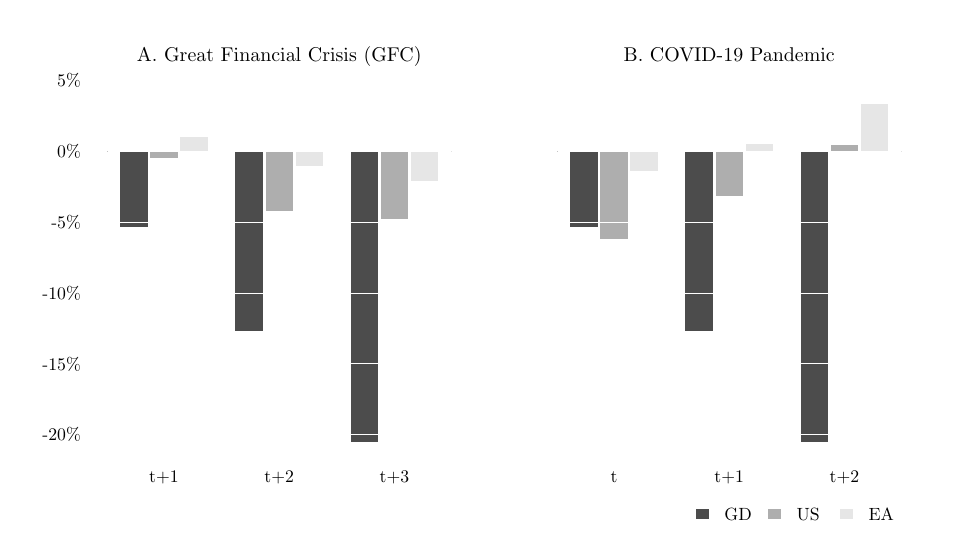
\begin{tikzpicture}[x=1pt,y=1pt]
\definecolor{fillColor}{RGB}{255,255,255}
\path[use as bounding box,fill=fillColor,fill opacity=0.00] (0,0) rectangle (325.21,180.67);
\begin{scope}
\path[clip] (  0.00,  0.00) rectangle (162.61,180.67);
\definecolor{fillColor}{gray}{0.30}

\path[fill=fillColor] ( 33.40,135.90) rectangle ( 43.31,108.47);
\definecolor{fillColor}{RGB}{174,174,174}

\path[fill=fillColor] ( 44.31,135.90) rectangle ( 54.22,133.50);
\definecolor{fillColor}{RGB}{230,230,230}

\path[fill=fillColor] ( 55.21,135.90) rectangle ( 65.13,141.05);
\definecolor{fillColor}{gray}{0.30}

\path[fill=fillColor] ( 75.04,135.90) rectangle ( 84.96, 70.99);
\definecolor{fillColor}{RGB}{174,174,174}

\path[fill=fillColor] ( 85.95,135.90) rectangle ( 95.86,114.29);
\definecolor{fillColor}{RGB}{230,230,230}

\path[fill=fillColor] ( 96.85,135.90) rectangle (106.77,130.64);
\definecolor{fillColor}{gray}{0.30}

\path[fill=fillColor] (116.68,135.90) rectangle (126.60, 30.87);
\definecolor{fillColor}{RGB}{174,174,174}

\path[fill=fillColor] (127.59,135.90) rectangle (137.50,111.44);
\definecolor{fillColor}{RGB}{230,230,230}

\path[fill=fillColor] (138.49,135.90) rectangle (148.41,125.35);
\end{scope}
\begin{scope}
\path[clip] (  0.00,  0.00) rectangle (325.21,180.67);
\definecolor{drawColor}{RGB}{0,0,0}

\node[text=drawColor,anchor=base,inner sep=0pt, outer sep=0pt, scale=  0.64] at ( 49.26, 16.32) {t+1};

\node[text=drawColor,anchor=base,inner sep=0pt, outer sep=0pt, scale=  0.64] at ( 90.90, 16.32) {t+2};

\node[text=drawColor,anchor=base,inner sep=0pt, outer sep=0pt, scale=  0.64] at (132.54, 16.32) {t+3};
\end{scope}
\begin{scope}
\path[clip] ( 28.80, 33.60) rectangle (153.01,161.47);
\definecolor{drawColor}{RGB}{0,0,0}

\path[draw=drawColor,line width= 0.4pt,line join=round,line cap=round] ( 28.80,135.90) -- (153.01,135.90);
\end{scope}
\begin{scope}
\path[clip] (  0.00,  0.00) rectangle (325.21,180.67);
\definecolor{drawColor}{RGB}{0,0,0}

\node[text=drawColor,anchor=base east,inner sep=0pt, outer sep=0pt, scale=  0.64] at ( 19.20, 31.40) {-20\%};

\node[text=drawColor,anchor=base east,inner sep=0pt, outer sep=0pt, scale=  0.64] at ( 19.20, 56.97) {-15\%};

\node[text=drawColor,anchor=base east,inner sep=0pt, outer sep=0pt, scale=  0.64] at ( 19.20, 82.55) {-10\%};

\node[text=drawColor,anchor=base east,inner sep=0pt, outer sep=0pt, scale=  0.64] at ( 19.20,108.12) {-5\%};

\node[text=drawColor,anchor=base east,inner sep=0pt, outer sep=0pt, scale=  0.64] at ( 19.20,133.70) {0\%};

\node[text=drawColor,anchor=base east,inner sep=0pt, outer sep=0pt, scale=  0.64] at ( 19.20,159.27) {5\%};
\end{scope}
\begin{scope}
\path[clip] ( 28.80, 33.60) rectangle (153.01,161.47);
\definecolor{drawColor}{RGB}{255,255,255}

\path[draw=drawColor,line width= 0.4pt,line join=round,line cap=round] ( 28.80, 33.60) -- (153.01, 33.60);

\path[draw=drawColor,line width= 0.4pt,line join=round,line cap=round] ( 28.80, 59.17) -- (153.01, 59.17);

\path[draw=drawColor,line width= 0.4pt,line join=round,line cap=round] ( 28.80, 84.75) -- (153.01, 84.75);

\path[draw=drawColor,line width= 0.4pt,line join=round,line cap=round] ( 28.80,110.33) -- (153.01,110.33);

\path[draw=drawColor,line width= 0.4pt,line join=round,line cap=round] ( 28.80,135.90) -- (153.01,135.90);

\path[draw=drawColor,line width= 0.4pt,line join=round,line cap=round] ( 28.80,161.47) -- (153.01,161.47);
\end{scope}
\begin{scope}
\path[clip] (  0.00,  0.00) rectangle (162.61,180.67);
\definecolor{drawColor}{RGB}{0,0,0}

\node[text=drawColor,anchor=base,inner sep=0pt, outer sep=0pt, scale=  0.72] at ( 90.90,168.60) {A. Great Financial Crisis (GFC)};
\end{scope}
\begin{scope}
\path[clip] (162.61,  0.00) rectangle (325.21,180.67);
\definecolor{fillColor}{gray}{0.30}

\path[fill=fillColor] (196.01,135.90) rectangle (205.92,108.47);
\definecolor{fillColor}{RGB}{174,174,174}

\path[fill=fillColor] (206.91,135.90) rectangle (216.83,104.27);
\definecolor{fillColor}{RGB}{230,230,230}

\path[fill=fillColor] (217.82,135.90) rectangle (227.73,128.84);
\definecolor{fillColor}{gray}{0.30}

\path[fill=fillColor] (237.65,135.90) rectangle (247.56, 70.99);
\definecolor{fillColor}{RGB}{174,174,174}

\path[fill=fillColor] (248.55,135.90) rectangle (258.47,119.80);
\definecolor{fillColor}{RGB}{230,230,230}

\path[fill=fillColor] (259.46,135.90) rectangle (269.37,138.54);
\definecolor{fillColor}{gray}{0.30}

\path[fill=fillColor] (279.29,135.90) rectangle (289.20, 30.87);
\definecolor{fillColor}{RGB}{174,174,174}

\path[fill=fillColor] (290.19,135.90) rectangle (300.11,138.34);
\definecolor{fillColor}{RGB}{230,230,230}

\path[fill=fillColor] (301.10,135.90) rectangle (311.01,152.93);
\end{scope}
\begin{scope}
\path[clip] (  0.00,  0.00) rectangle (325.21,180.67);
\definecolor{drawColor}{RGB}{0,0,0}

\node[text=drawColor,anchor=base,inner sep=0pt, outer sep=0pt, scale=  0.64] at (211.87, 16.32) {t};

\node[text=drawColor,anchor=base,inner sep=0pt, outer sep=0pt, scale=  0.64] at (253.51, 16.32) {t+1};

\node[text=drawColor,anchor=base,inner sep=0pt, outer sep=0pt, scale=  0.64] at (295.15, 16.32) {t+2};
\end{scope}
\begin{scope}
\path[clip] (191.41, 33.60) rectangle (315.62,161.47);
\definecolor{drawColor}{RGB}{0,0,0}

\path[draw=drawColor,line width= 0.4pt,line join=round,line cap=round] (191.41,135.90) -- (315.62,135.90);
\definecolor{drawColor}{RGB}{255,255,255}

\path[draw=drawColor,line width= 0.4pt,line join=round,line cap=round] (191.41, 33.60) -- (315.62, 33.60);

\path[draw=drawColor,line width= 0.4pt,line join=round,line cap=round] (191.41, 59.17) -- (315.62, 59.17);

\path[draw=drawColor,line width= 0.4pt,line join=round,line cap=round] (191.41, 84.75) -- (315.62, 84.75);

\path[draw=drawColor,line width= 0.4pt,line join=round,line cap=round] (191.41,110.33) -- (315.62,110.33);

\path[draw=drawColor,line width= 0.4pt,line join=round,line cap=round] (191.41,135.90) -- (315.62,135.90);

\path[draw=drawColor,line width= 0.4pt,line join=round,line cap=round] (191.41,161.47) -- (315.62,161.47);
\end{scope}
\begin{scope}
\path[clip] (162.61,  0.00) rectangle (325.21,180.67);
\definecolor{fillColor}{gray}{0.30}

\path[fill=fillColor] (241.43,  6.87) rectangle (246.03,  3.03);
\definecolor{fillColor}{RGB}{174,174,174}

\path[fill=fillColor] (267.46,  6.87) rectangle (272.07,  3.03);
\definecolor{fillColor}{RGB}{230,230,230}

\path[fill=fillColor] (293.50,  6.87) rectangle (298.11,  3.03);
\definecolor{drawColor}{RGB}{0,0,0}

\node[text=drawColor,anchor=base west,inner sep=0pt, outer sep=0pt, scale=  0.64] at (251.79,  2.74) {GD};

\node[text=drawColor,anchor=base west,inner sep=0pt, outer sep=0pt, scale=  0.64] at (277.83,  2.74) {US};

\node[text=drawColor,anchor=base west,inner sep=0pt, outer sep=0pt, scale=  0.64] at (303.87,  2.74) {EA};

\node[text=drawColor,anchor=base,inner sep=0pt, outer sep=0pt, scale=  0.72] at (253.51,168.60) {B. COVID-19 Pandemic};
\end{scope}
\end{tikzpicture}

\end{figure} 
	
\end{frame}

\begin{frame}{Stock Markets Post GFC and COVID-19 Pandemic}

\begin{figure}[h!]
     \centering
     % Created by tikzDevice version 0.12.5 on 2023-11-24 23:42:35
% !TEX encoding = UTF-8 Unicode
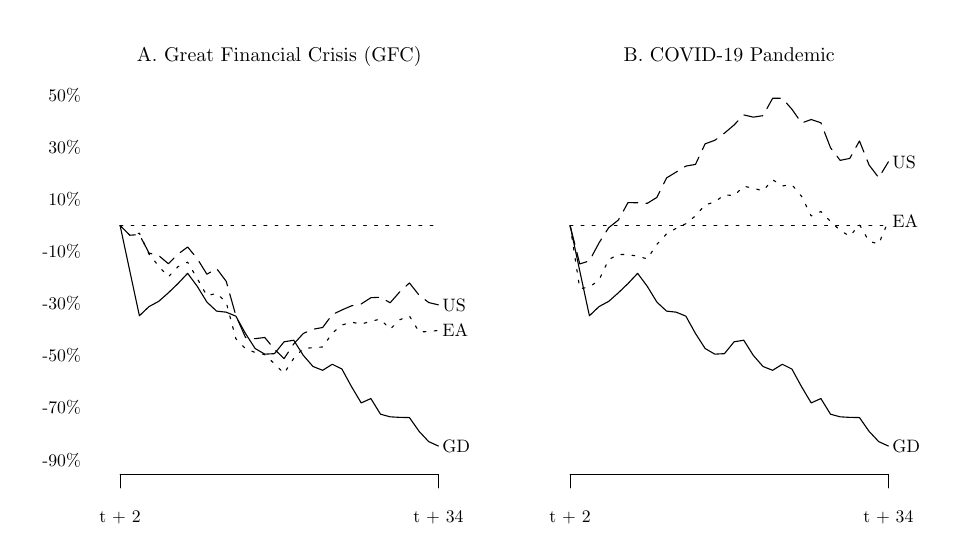
\begin{tikzpicture}[x=1pt,y=1pt]
\definecolor{fillColor}{RGB}{255,255,255}
\path[use as bounding box,fill=fillColor,fill opacity=0.00] (0,0) rectangle (325.21,180.67);
\begin{scope}
\path[clip] ( 28.80, 19.20) rectangle (153.01,161.47);
\definecolor{drawColor}{RGB}{0,0,0}

\path[draw=drawColor,line width= 0.4pt,line join=round,line cap=round] ( 33.40,109.16) --
	( 36.89, 92.80) --
	( 40.37, 76.57) --
	( 43.86, 79.89) --
	( 47.34, 81.77) --
	( 50.83, 84.85) --
	( 54.31, 88.20) --
	( 57.80, 91.91) --
	( 61.28, 87.20) --
	( 64.77, 81.50) --
	( 68.25, 78.25) --
	( 71.74, 77.87) --
	( 75.22, 76.43) --
	( 78.71, 70.16) --
	( 82.19, 64.73) --
	( 85.68, 62.70) --
	( 89.16, 62.87) --
	( 92.65, 67.15) --
	( 96.13, 67.74) --
	( 99.62, 62.23) --
	(103.10, 58.24) --
	(106.59, 56.86) --
	(110.07, 59.04) --
	(113.56, 57.30) --
	(117.04, 50.91) --
	(120.53, 45.07) --
	(124.01, 46.66) --
	(127.50, 41.00) --
	(130.98, 40.05) --
	(134.47, 39.85) --
	(137.95, 39.78) --
	(141.44, 34.80) --
	(144.92, 31.08) --
	(148.41, 29.50);
\end{scope}
\begin{scope}
\path[clip] ( 28.80, 19.20) rectangle (153.01,161.47);
\definecolor{drawColor}{RGB}{0,0,0}

\path[draw=drawColor,line width= 0.4pt,dash pattern=on 1pt off 3pt ,line join=round,line cap=round] ( 33.40,109.16) --
	(148.41,109.16);
\end{scope}
\begin{scope}
\path[clip] (  0.00,  0.00) rectangle (325.21,180.67);
\definecolor{drawColor}{RGB}{0,0,0}

\path[draw=drawColor,line width= 0.4pt,line join=round,line cap=round] ( 33.40, 19.20) -- (148.41, 19.20);

\path[draw=drawColor,line width= 0.4pt,line join=round,line cap=round] ( 33.40, 19.20) -- ( 33.40, 14.40);

\path[draw=drawColor,line width= 0.4pt,line join=round,line cap=round] (148.41, 19.20) -- (148.41, 14.40);

\node[text=drawColor,anchor=base,inner sep=0pt, outer sep=0pt, scale=  0.64] at ( 33.40,  1.92) {t + 2};

\node[text=drawColor,anchor=base,inner sep=0pt, outer sep=0pt, scale=  0.64] at (148.41,  1.92) {t + 34};

\node[text=drawColor,anchor=base east,inner sep=0pt, outer sep=0pt, scale=  0.64] at ( 19.20, 22.27) {-90\%};

\node[text=drawColor,anchor=base east,inner sep=0pt, outer sep=0pt, scale=  0.64] at ( 19.20, 41.08) {-70\%};

\node[text=drawColor,anchor=base east,inner sep=0pt, outer sep=0pt, scale=  0.64] at ( 19.20, 59.90) {-50\%};

\node[text=drawColor,anchor=base east,inner sep=0pt, outer sep=0pt, scale=  0.64] at ( 19.20, 78.72) {-30\%};

\node[text=drawColor,anchor=base east,inner sep=0pt, outer sep=0pt, scale=  0.64] at ( 19.20, 97.54) {-10\%};

\node[text=drawColor,anchor=base east,inner sep=0pt, outer sep=0pt, scale=  0.64] at ( 19.20,116.36) {10\%};

\node[text=drawColor,anchor=base east,inner sep=0pt, outer sep=0pt, scale=  0.64] at ( 19.20,135.18) {30\%};

\node[text=drawColor,anchor=base east,inner sep=0pt, outer sep=0pt, scale=  0.64] at ( 19.20,154.00) {50\%};

\node[text=drawColor,anchor=base west,inner sep=0pt, outer sep=0pt, scale=  0.65] at (149.84, 27.27) {GD};
\end{scope}
\begin{scope}
\path[clip] ( 28.80, 19.20) rectangle (153.01,161.47);
\definecolor{drawColor}{RGB}{0,0,0}

\path[draw=drawColor,line width= 0.4pt,dash pattern=on 7pt off 3pt ,line join=round,line cap=round] ( 33.40,109.16) --
	( 36.89,105.67) --
	( 40.37,105.89) --
	( 43.86, 99.22) --
	( 47.34, 98.33) --
	( 50.83, 95.38) --
	( 54.31, 98.82) --
	( 57.80,101.41) --
	( 61.28, 97.20) --
	( 64.77, 91.57) --
	( 68.25, 93.65) --
	( 71.74, 89.02) --
	( 75.22, 76.66) --
	( 78.71, 68.73) --
	( 82.19, 68.30) --
	( 85.68, 68.72) --
	( 89.16, 64.46) --
	( 92.65, 61.09) --
	( 96.13, 66.38) --
	( 99.62, 70.19) --
	(103.10, 71.69) --
	(106.59, 72.33) --
	(110.07, 77.00) --
	(113.56, 78.66) --
	(117.04, 80.17) --
	(120.53, 80.84) --
	(124.01, 83.09) --
	(127.50, 83.26) --
	(130.98, 81.26) --
	(134.47, 85.23) --
	(137.95, 88.43) --
	(141.44, 84.00) --
	(144.92, 81.35) --
	(148.41, 80.50);
\end{scope}
\begin{scope}
\path[clip] (  0.00,  0.00) rectangle (325.21,180.67);
\definecolor{drawColor}{RGB}{0,0,0}

\node[text=drawColor,anchor=base west,inner sep=0pt, outer sep=0pt, scale=  0.65] at (149.84, 78.27) {US};
\end{scope}
\begin{scope}
\path[clip] ( 28.80, 19.20) rectangle (153.01,161.47);
\definecolor{drawColor}{RGB}{0,0,0}

\path[draw=drawColor,line width= 0.4pt,dash pattern=on 1pt off 3pt ,line join=round,line cap=round] ( 33.40,109.16) --
	( 36.89,105.70) --
	( 40.37,106.38) --
	( 43.86, 98.82) --
	( 47.34, 94.51) --
	( 50.83, 90.61) --
	( 54.31, 94.29) --
	( 57.80, 95.95) --
	( 61.28, 90.01) --
	( 64.77, 83.78) --
	( 68.25, 84.70) --
	( 71.74, 81.45) --
	( 75.22, 68.28) --
	( 78.71, 64.64) --
	( 82.19, 63.31) --
	( 85.68, 62.54) --
	( 89.16, 59.21) --
	( 92.65, 55.74) --
	( 96.13, 61.17) --
	( 99.62, 64.80) --
	(103.10, 65.01) --
	(106.59, 65.30) --
	(110.07, 70.30) --
	(113.56, 73.22) --
	(117.04, 74.27) --
	(120.53, 73.54) --
	(124.01, 74.60) --
	(127.50, 75.34) --
	(130.98, 71.69) --
	(134.47, 75.13) --
	(137.95, 76.50) --
	(141.44, 70.74) --
	(144.92, 70.85) --
	(148.41, 71.27);
\end{scope}
\begin{scope}
\path[clip] (  0.00,  0.00) rectangle (325.21,180.67);
\definecolor{drawColor}{RGB}{0,0,0}

\node[text=drawColor,anchor=base west,inner sep=0pt, outer sep=0pt, scale=  0.65] at (149.84, 69.04) {EA};
\end{scope}
\begin{scope}
\path[clip] (  0.00,  0.00) rectangle (162.61,180.67);
\definecolor{drawColor}{RGB}{0,0,0}

\node[text=drawColor,anchor=base,inner sep=0pt, outer sep=0pt, scale=  0.72] at ( 90.90,168.60) {A. Great Financial Crisis (GFC)};
\end{scope}
\begin{scope}
\path[clip] (191.41, 19.20) rectangle (315.62,161.47);
\definecolor{drawColor}{RGB}{0,0,0}

\path[draw=drawColor,line width= 0.4pt,line join=round,line cap=round] (196.01,109.16) --
	(199.49, 92.80) --
	(202.98, 76.57) --
	(206.46, 79.89) --
	(209.95, 81.77) --
	(213.43, 84.85) --
	(216.92, 88.20) --
	(220.40, 91.91) --
	(223.89, 87.20) --
	(227.37, 81.50) --
	(230.86, 78.25) --
	(234.34, 77.87) --
	(237.83, 76.43) --
	(241.31, 70.16) --
	(244.80, 64.73) --
	(248.28, 62.70) --
	(251.77, 62.87) --
	(255.25, 67.15) --
	(258.74, 67.74) --
	(262.22, 62.23) --
	(265.71, 58.24) --
	(269.19, 56.86) --
	(272.68, 59.04) --
	(276.16, 57.30) --
	(279.65, 50.91) --
	(283.13, 45.07) --
	(286.62, 46.66) --
	(290.10, 41.00) --
	(293.59, 40.05) --
	(297.07, 39.85) --
	(300.56, 39.78) --
	(304.04, 34.80) --
	(307.53, 31.08) --
	(311.01, 29.50);
\end{scope}
\begin{scope}
\path[clip] (191.41, 19.20) rectangle (315.62,161.47);
\definecolor{drawColor}{RGB}{0,0,0}

\path[draw=drawColor,line width= 0.4pt,dash pattern=on 1pt off 3pt ,line join=round,line cap=round] (196.01,109.16) --
	(311.01,109.16);
\end{scope}
\begin{scope}
\path[clip] (  0.00,  0.00) rectangle (325.21,180.67);
\definecolor{drawColor}{RGB}{0,0,0}

\path[draw=drawColor,line width= 0.4pt,line join=round,line cap=round] (196.01, 19.20) -- (311.01, 19.20);

\path[draw=drawColor,line width= 0.4pt,line join=round,line cap=round] (196.01, 19.20) -- (196.01, 14.40);

\path[draw=drawColor,line width= 0.4pt,line join=round,line cap=round] (311.01, 19.20) -- (311.01, 14.40);

\node[text=drawColor,anchor=base,inner sep=0pt, outer sep=0pt, scale=  0.64] at (196.01,  1.92) {t + 2};

\node[text=drawColor,anchor=base,inner sep=0pt, outer sep=0pt, scale=  0.64] at (311.01,  1.92) {t + 34};

\node[text=drawColor,anchor=base west,inner sep=0pt, outer sep=0pt, scale=  0.65] at (312.45, 27.27) {GD};
\end{scope}
\begin{scope}
\path[clip] (191.41, 19.20) rectangle (315.62,161.47);
\definecolor{drawColor}{RGB}{0,0,0}

\path[draw=drawColor,line width= 0.4pt,dash pattern=on 7pt off 3pt ,line join=round,line cap=round] (196.01,109.16) --
	(199.49, 95.29) --
	(202.98, 96.40) --
	(206.46,102.92) --
	(209.95,108.40) --
	(213.43,111.14) --
	(216.92,117.44) --
	(220.40,117.41) --
	(223.89,117.20) --
	(227.37,119.34) --
	(230.86,126.39) --
	(234.34,128.49) --
	(237.83,130.64) --
	(241.31,131.27) --
	(244.80,138.70) --
	(248.28,139.96) --
	(251.77,142.55) --
	(255.25,145.50) --
	(258.74,149.14) --
	(262.22,148.34) --
	(265.71,148.87) --
	(269.19,155.15) --
	(272.68,155.15) --
	(276.16,151.19) --
	(279.65,146.21) --
	(283.13,147.49) --
	(286.62,146.32) --
	(290.10,137.29) --
	(293.59,132.72) --
	(297.07,133.43) --
	(300.56,139.73) --
	(304.04,131.05) --
	(307.53,126.44) --
	(311.01,132.18);
\end{scope}
\begin{scope}
\path[clip] (  0.00,  0.00) rectangle (325.21,180.67);
\definecolor{drawColor}{RGB}{0,0,0}

\node[text=drawColor,anchor=base west,inner sep=0pt, outer sep=0pt, scale=  0.65] at (312.45,129.93) {US};
\end{scope}
\begin{scope}
\path[clip] (191.41, 19.20) rectangle (315.62,161.47);
\definecolor{drawColor}{RGB}{0,0,0}

\path[draw=drawColor,line width= 0.4pt,dash pattern=on 1pt off 3pt ,line join=round,line cap=round] (196.01,109.16) --
	(199.49, 86.36) --
	(202.98, 86.90) --
	(206.46, 89.50) --
	(209.95, 96.86) --
	(213.43, 98.73) --
	(216.92, 98.69) --
	(220.40, 98.08) --
	(223.89, 97.13) --
	(227.37,102.37) --
	(230.86,106.16) --
	(234.34,108.18) --
	(237.83,109.83) --
	(241.31,112.68) --
	(244.80,116.67) --
	(248.28,117.65) --
	(251.77,120.30) --
	(255.25,119.96) --
	(258.74,123.36) --
	(262.22,122.66) --
	(265.71,121.70) --
	(269.19,125.72) --
	(272.68,123.48) --
	(276.16,123.93) --
	(279.65,119.70) --
	(283.13,112.62) --
	(286.62,114.23) --
	(290.10,110.64) --
	(293.59,107.42) --
	(297.07,105.29) --
	(300.56,109.49) --
	(304.04,103.44) --
	(307.53,102.55) --
	(311.01,110.80);
\end{scope}
\begin{scope}
\path[clip] (  0.00,  0.00) rectangle (325.21,180.67);
\definecolor{drawColor}{RGB}{0,0,0}

\node[text=drawColor,anchor=base west,inner sep=0pt, outer sep=0pt, scale=  0.65] at (312.45,108.56) {EA};
\end{scope}
\begin{scope}
\path[clip] (162.61,  0.00) rectangle (325.21,180.67);
\definecolor{drawColor}{RGB}{0,0,0}

\node[text=drawColor,anchor=base,inner sep=0pt, outer sep=0pt, scale=  0.72] at (253.51,168.60) {B. COVID-19 Pandemic};
\end{scope}
\end{tikzpicture}

\end{figure} 
	
\end{frame}

\section{Resources}

\begin{frame}{Data and Code for Research Reproducibility}

GitHub repository: 

\quad \quad \textit{https://github.com/lyuben-ivanov/lille23}

\vfill

\texttt{R} installation of package \texttt{lille23}:

\quad \quad \textit{devtools::install\_github(``lyuben-ivanov/lille23")}

\end{frame}



\begin{frame}
\centering \Huge \bfseries Thank you!	
\end{frame}

\end{document}











